%% TeXworks instructions:
% !TeX root = ./report.tex
% !TEX encoding = UTF-8 Unicode
%% !TEX program = arara
%% !TEX TS-program = arara
% !TeX spellcheck = it-IT

% arara: pdflatex: { synctex: yes, action: batchmode, options: "-halt-on-error -file-line-error-style" }
% arara: pdflatex: { synctex: yes, action: nonstopmode, options: "-halt-on-error -file-line-error-style" }

%% Generate a report.xmpdata file with title and authors for PDF/A-compliant format %%
\begin{filecontents*}{\jobname.xmpdata}
    \Title{Maraph1-mp Project Report}
    \Author{Nicholas Brasini\sep Gjulio Jakova\sep Federico Naldini\sep Jacopo Riciputi}
\end{filecontents*}

\documentclass[%
    a4paper,            % specifica il formato A4 (default: letter)
    10pt,               % specifica la dimensione del carattere a 10
    oneside,            % serve per impaginare per stampa solo fronte
    notitlepage         % mette il titolo in una pagina separata (solo per article)
]{article}

\usepackage{a4wide}             % consente di avere più spazio nell'A4

%% ORDINE IMPORTANTE INIZIO %%%%%%%%%%%%
\usepackage[T1]{fontenc}        % serve per impostare la codifica di output del font
\usepackage{textcomp}           % serve per fornire supporto ai Text Companion fonts
\usepackage[utf8]{inputenc}     % serve per impostare la codifica di input del font
\usepackage[
    english,            % utilizza l'inglese come lingua secondaria
    italian             % utilizza l'italiano come lingua primaria
]{babel}                        % serve per scrivere Indice, Capitolo, etc in Italiano

\usepackage{lmodern}            % carica una variante Latin Modern prodotto dal GUST
%% ORDINE IMPORTANTE FINE %%%%%%%%%%%%%%

\usepackage{indentfirst}        % serve per avere l'indentazione nel primo paragrafo
\usepackage{setspace}           % serve a fornire comandi di interlinea standard
\usepackage{xcolor}             % serve per la gestione dei colori nel testo
\usepackage{graphicx}           % serve per includere immagini e grafici

\graphicspath{{./images/}}

\usepackage[%
    strict,             % rende tutti gli warning degli errori
    autostyle,          % imposta lo stile in base al linguaggio specificato in babel
    english=american,   % imposta lo stile per l'inglese
    italian=guillemets  % imposta lo stile per l'italiano
]{csquotes}                     % serve a impostare lo stile delle virgolette

\usepackage{multirow}           % aggiunge la possibilità di raggruppare celle su più righe nelle tabelle

\onehalfspacing%                % Imposta interlinea a 1,5 ed equivale a \linespread{1,5}

\setcounter{secnumdepth}{4}     % Numera fino alla sottosezione nel corpo del testo
\setcounter{tocdepth}{4}        % Numera fino alla sotto-sottosezione nell'indice

\usepackage[%
    depth=3,            % equivale a bookmarksdepth di hyperref
    open=false,         % equivale a bookmarksopen di hyperref
    numbered=true       % equivale a bookmarksnumbered di hyperref
]{bookmark}                     % Gestisce i segnalibri meglio di hyperref
\usepackage{hyperref}           % Gestisce tutte le cose ipertestuali del pdf
\hypersetup{%
    pdfpagemode={UseNone},
    hidelinks,          % nasconde i collegamenti (non vengono quadrettati)
    hypertexnames=false,
    linktoc=all,        % inserisce i link nell'indice
    unicode=true,       % only Latin characters in Acrobat’s bookmarks
    pdftoolbar=false,   % show Acrobat’s toolbar?
    pdfmenubar=false,   % show Acrobat’s menu?
    plainpages=false,
    breaklinks,
    pdfstartview={Fit},
    pdfauthor={Nicholas Brasini, Gjulio Jakova, Federico Naldini, Jacopo Riciputi},
    pdfcreator={Nicholas Brasini, Gjulio Jakova, Federico Naldini, Jacopo Riciputi},
    pdftitle={Maraph1-mp Project Report},
    pdflang={it}
}
\usepackage[utf8]{inputenc} % serve per avere l'indice di tutti i capitoli all'inizio 

%\usepackage[a-1b]{pdfx}
\usepackage[%
    english,italian,    % definizione delle lingue da usare
    nameinlink          % inserisce i link nei riferimenti
]{cleveref}                     % permette di usare riferimenti migliori dei \ref e dei varioref

\title{\LARGE{\textbf{Maraph1-mp Project Report}}}

\author{%
    Nicholas~Brasini\\%
    Gjulio~Jakova\\%
    Federico~Naldini\\%
    Jacopo~Riciputi
}

\date{%
    \small{Paradigmi di Programmazione e Sviluppo}\\%
    \small{Anni accademici 2017--2018 e 2018--2019}
}


\begin{document}
	
    \maketitle
    \clearpage
	\tableofcontents
	\clearpage
    \section*{\Huge {Capitolo 1}\label{chapter1}}
      \section{Processo di sviluppo}\label{sec:process}
        \subsection {Metodologia di sviluppo}\label{subsec:metodology}
        \subsection {Strumenti adottati}\label{subsec:tools}
        
        \clearpage
        
    \section*{\Huge {\textbf Capitolo 2}\label{chapter2}}
    \section{Requisiti}\label{sec:requirements}
         \subsection {Requisiti utente}\label{subsec:requirements:business}
             \subsection {Requisiti funzionali}\label{subsec:requirements:functional}
            \subsubsection[Gioco]{\large {Regole del gioco}\label{subsub:requirements:game}}
            \subsubsection[NoAutenticazion]{\large {Servizio di gioco senza autenticazione}\label{subsub:requirements:noauth}}
            \subsubsection[Autenticazion]{\large {Servizio di gioco con autenticazione}\label{subsub:requirements:auth}}
            \subsubsection[Stanze di gioco]{\large {Servizio delle stanze di gioco}\label{subsub:requirements:lobby}}
            \subsubsection[Interfaccia utente]{\large {Interfaccia grafica per l'utente}\label{subsub:requirements:gui}}
        \subsection {Requisiti non funzionali}\label{subsec:requirements:notFunctional}
        \subsection {Requisiti implementativi}\label{subsec:requirements:implementative}
   
   \clearpage
    \section*{\Huge {\textbf Capitolo 3}\label{chapter3}}
    \section{Design architetturale}\label{sec:design}
        L'architettura del sistema si basa fortemente su un design client-server. 
        Mentre per la realizzazione dell'applicazione locale è stato adottato il pattern Model-View-Controller, così da permettere una maggior suddivisione dei compiti, soprattuto per quanto riguarda la parte grafica e logica del gioco dalla sezione di interazione con il remoto. 
        Per il lato server-side invece, dato che le specifiche, oltre che a richiedere una parte statica, di semplice gestione dati, richiedevano anche una parte dinamica (real-time), sono stati adottati due differenti pattern. La gestione dei dati è stata affidata ad un server che mette a disposizione per i client una serie di chiamate \textbf{API REST}, mentre per il real-time la scelta è ricaduta sulla creazione di una sessione di gioco utilizzando il pattern \textbf{Publish-Subscribe}.
        
        
        
        \subsection[Architettura]{Architettura e pattern utilizzati}\label{subsec:architecture}
            \subsubsection{Architettura server-side}\label{subsub:architecture:server}
            Nonostante l'architettura del server non sia a microservizi, si è preso spunto dalle loro potenzialità per costruire un modello che sia in futuro facilmente scalabile. 
            \\
            Per fare ciò è stato inserito tra il client e il backend un \textbf{Service discovery}. 
            
            \begin{figure}[h!]
                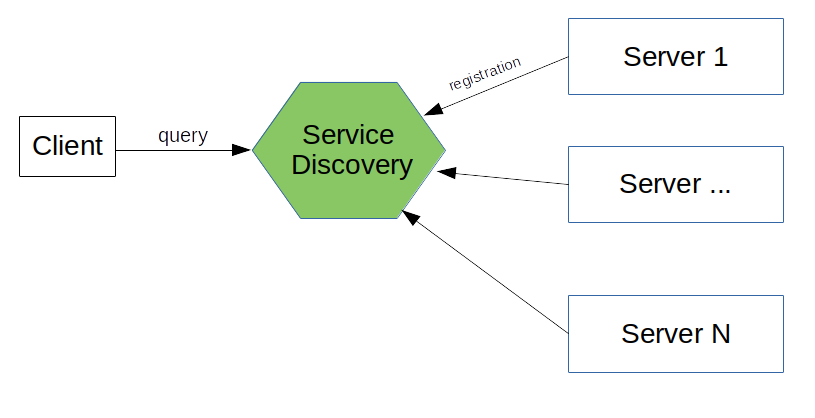
\includegraphics[width=\linewidth]{image/ArchitetturaDiscovery.png}
                \caption{Architettura client-server con Service Discovery}
            \end{figure}

            Grazie al Discovery è stata data, a livello di modello, la possibilità all'applicazione di aggiungere servizi e di avere anche più server che si occupano dello stesso, dato che, essendo il discovery l'intermediario tra il client e il server viene sfuttato anche come Load Balancer, andando perciò a indirizzare il client verso il servizio con meno carico al momento della chiamata.
            In questo modo l'applicazione risulta essere altamente scalibile oltre che fornire high availability e una buona tolleranza al fallimento. 
            \\
            Una volta ottenuto un instradamento verso uno dei server disponibili entra in gioco un classico servizio ad API REST che si occupa della gestione dell'utente, sia per la parte social che per la ricerca di una partita. 
            
            A questo punto l'architettura utilizzata cambia. Le richieste del dominio impongono una sessione di gioco attiva capace di mantenere uno stato e le API REST non risultano la miglior soluzione. 
            Per la costruzione di un dialogo in real-time fra tutti i componenti di una partita e il server, che gioca nel ruolo di manager di quest'ultima è stato adottato, come anticipato, il pattern Publish-Subscribe. 
            In questo modo ogni membro della partita in ascolto sul un determinato canale sono capaci di ricevere ed emettere messaggi cosicché alla produzione di un dato da parte di uno dei partecipanti, tutti gli altri siano capaci di recepirlo e di consumarlo per poi eventualmente rispondere tramite una determinata azione.
            
            \subsubsection{Architettura client-side}\label{subsub:architecture:client}
        \subsection{Tecnologie}\label{subsec:technologies}
        
        \clearpage
        
    \section{Design di dettaglio}\label{sec:design:details}
    
    \clearpage
    
    \section{Implementazione}\label{sec:implementation}
        \subsection{Nicholas Brasini}\label{subsec:brasini}
        \subsection{Gjulio Jakova}\label{subsec:jakova}
        \subsection{Federico Naldini}\label{subsec:naldini}
        \subsection{Jacopo Riciputi}\label{subsec:riciputi}
        
        \clearpage
        
    \section{Retrospettiva}\label{sec:retrospective}

\end{document}
